\documentclass[12pt,reqno, margin=1in]{amsart}

\usepackage{amsthm,amsmath,amssymb}
\usepackage{geometry}
\usepackage{mathtools}
\usepackage{proof}
\usepackage{xcolor}
\usepackage[T1]{fontenc}
\usepackage{courier}
\usepackage{hyperref}
\hypersetup{
    hidelinks=true
}
\usepackage{listings}
\lstset{basicstyle=\ttfamily\small, columns=fullflexible, language=Lisp, morekeywords={define, lambda, if, car, cdr, zero, eopl}, keywordstyle=\bfseries\color{blue!40!black}}
\newcommand{\code}[1]{\texttt{#1}}
 \geometry{
 a4paper,
 total={170mm,257mm},
 left=20mm, % so that the rule of inference can fit!
 top=20mm,
 }

\begin{document}

\begin{center}
\large\textbf{Problem Set 3 \\ COMP301 Fall 2019} \\
\normalsize\textbf{17.10.2019 17:30 - 18:45} \\
\end{center}

\vspace{7.5mm}

\textbf{Problem 1}\footnote{EOPL p.70 Exercise 3.4}:
Let $\text{\code{p}} = [\text{\code{x}} = \lceil33\rceil, \text{\code{y}}=\lceil22\rceil]$ \\
The derivation is:\\

\tiny

\infer{\code{(value-of <<if zero?(-(x, 11)) then -(y, 2) else -(y, 4)>>  p)= 18}}{\infer{\code{(value-of <<if zero?(-(x, 11)) then -(y, 2) else -(y, 4)>>  p)=(value-of <<-(y, 4)>> p)}}{\infer{\code{(value-of <<zero?(-(x, 11))>> p) = (bool-val \#f)}}{\infer{\code{(value-of <<-(x,11)>> p) = 22}}{\code{(value-of <<x>> p) = 33}}}} & \infer{\code{(value-of <<(-y, 4)>> p)=18}}{ \code{(value-of <<y>> p) = 22}}}

\normalsize
\vspace{7.5mm}

\textbf{Problem 2}\footnote{EOPL p.54 Exercise 2.27}:  Draw the abstract syntax tree for the lambda calculus expressions:
\begin{lstlisting}
((lambda (a) (a b)) c)
\end{lstlisting}
\code{app-exp} \\
$\xrightarrow{}$\code{lambda-exp   var-exp} \\
$\xrightarrow{}$\code{a  app-exp  c} \\
$\xrightarrow{}$\code{var-exp  var-exp} \\
$\xrightarrow{}$\code{a  c} \\
\begin{centering}
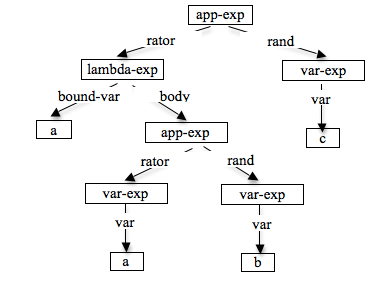
\includegraphics[width=0.8\textwidth]{PS3Q1P1.PNG}
\end{centering}

\newpage
\begin{lstlisting}
(lambda (x)
    (lambda (y)
        ((lambda (x)
            (x y))
        x)))
\end{lstlisting}
\code{lambda-exp} \\
$\xrightarrow{}$\code{x   lambda-exp} \\
$\xrightarrow{}$\code{y  app-exp} \\
$\xrightarrow{}$\code{lambda-exp  var-exp} \\
$\xrightarrow{}$\code{x  app-exp  x} \\
$\xrightarrow{}$\code{var-exp  var-exp} \\
$\xrightarrow{}$\code{x  y} \\
\begin{centering}
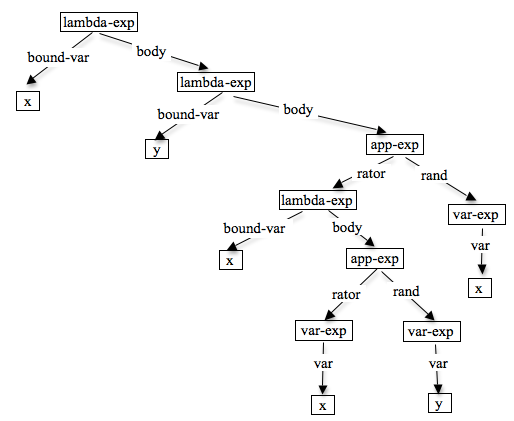
\includegraphics[width=0.8\textwidth]{PS3Q1P2.PNG}
\end{centering}

\end{document}